\section{Evaluation by examples (1.5 pages)}
\label{section:evaluation}

{\color{red} Welche Beispiele kommen hier?}

In the following we evaluate the proposed approach to multi-domain system modeling and systematic parameter variation using a number of examples. First we describe the examples in Section~\ref{section:examples} before discussing various issues in Section~\ref{section:discussion}.

\subsection{Examples}
\label{section:examples}

\begin{figure*}[t]
	\centering
	
	\begin{subfigure}{\columnwidth}
		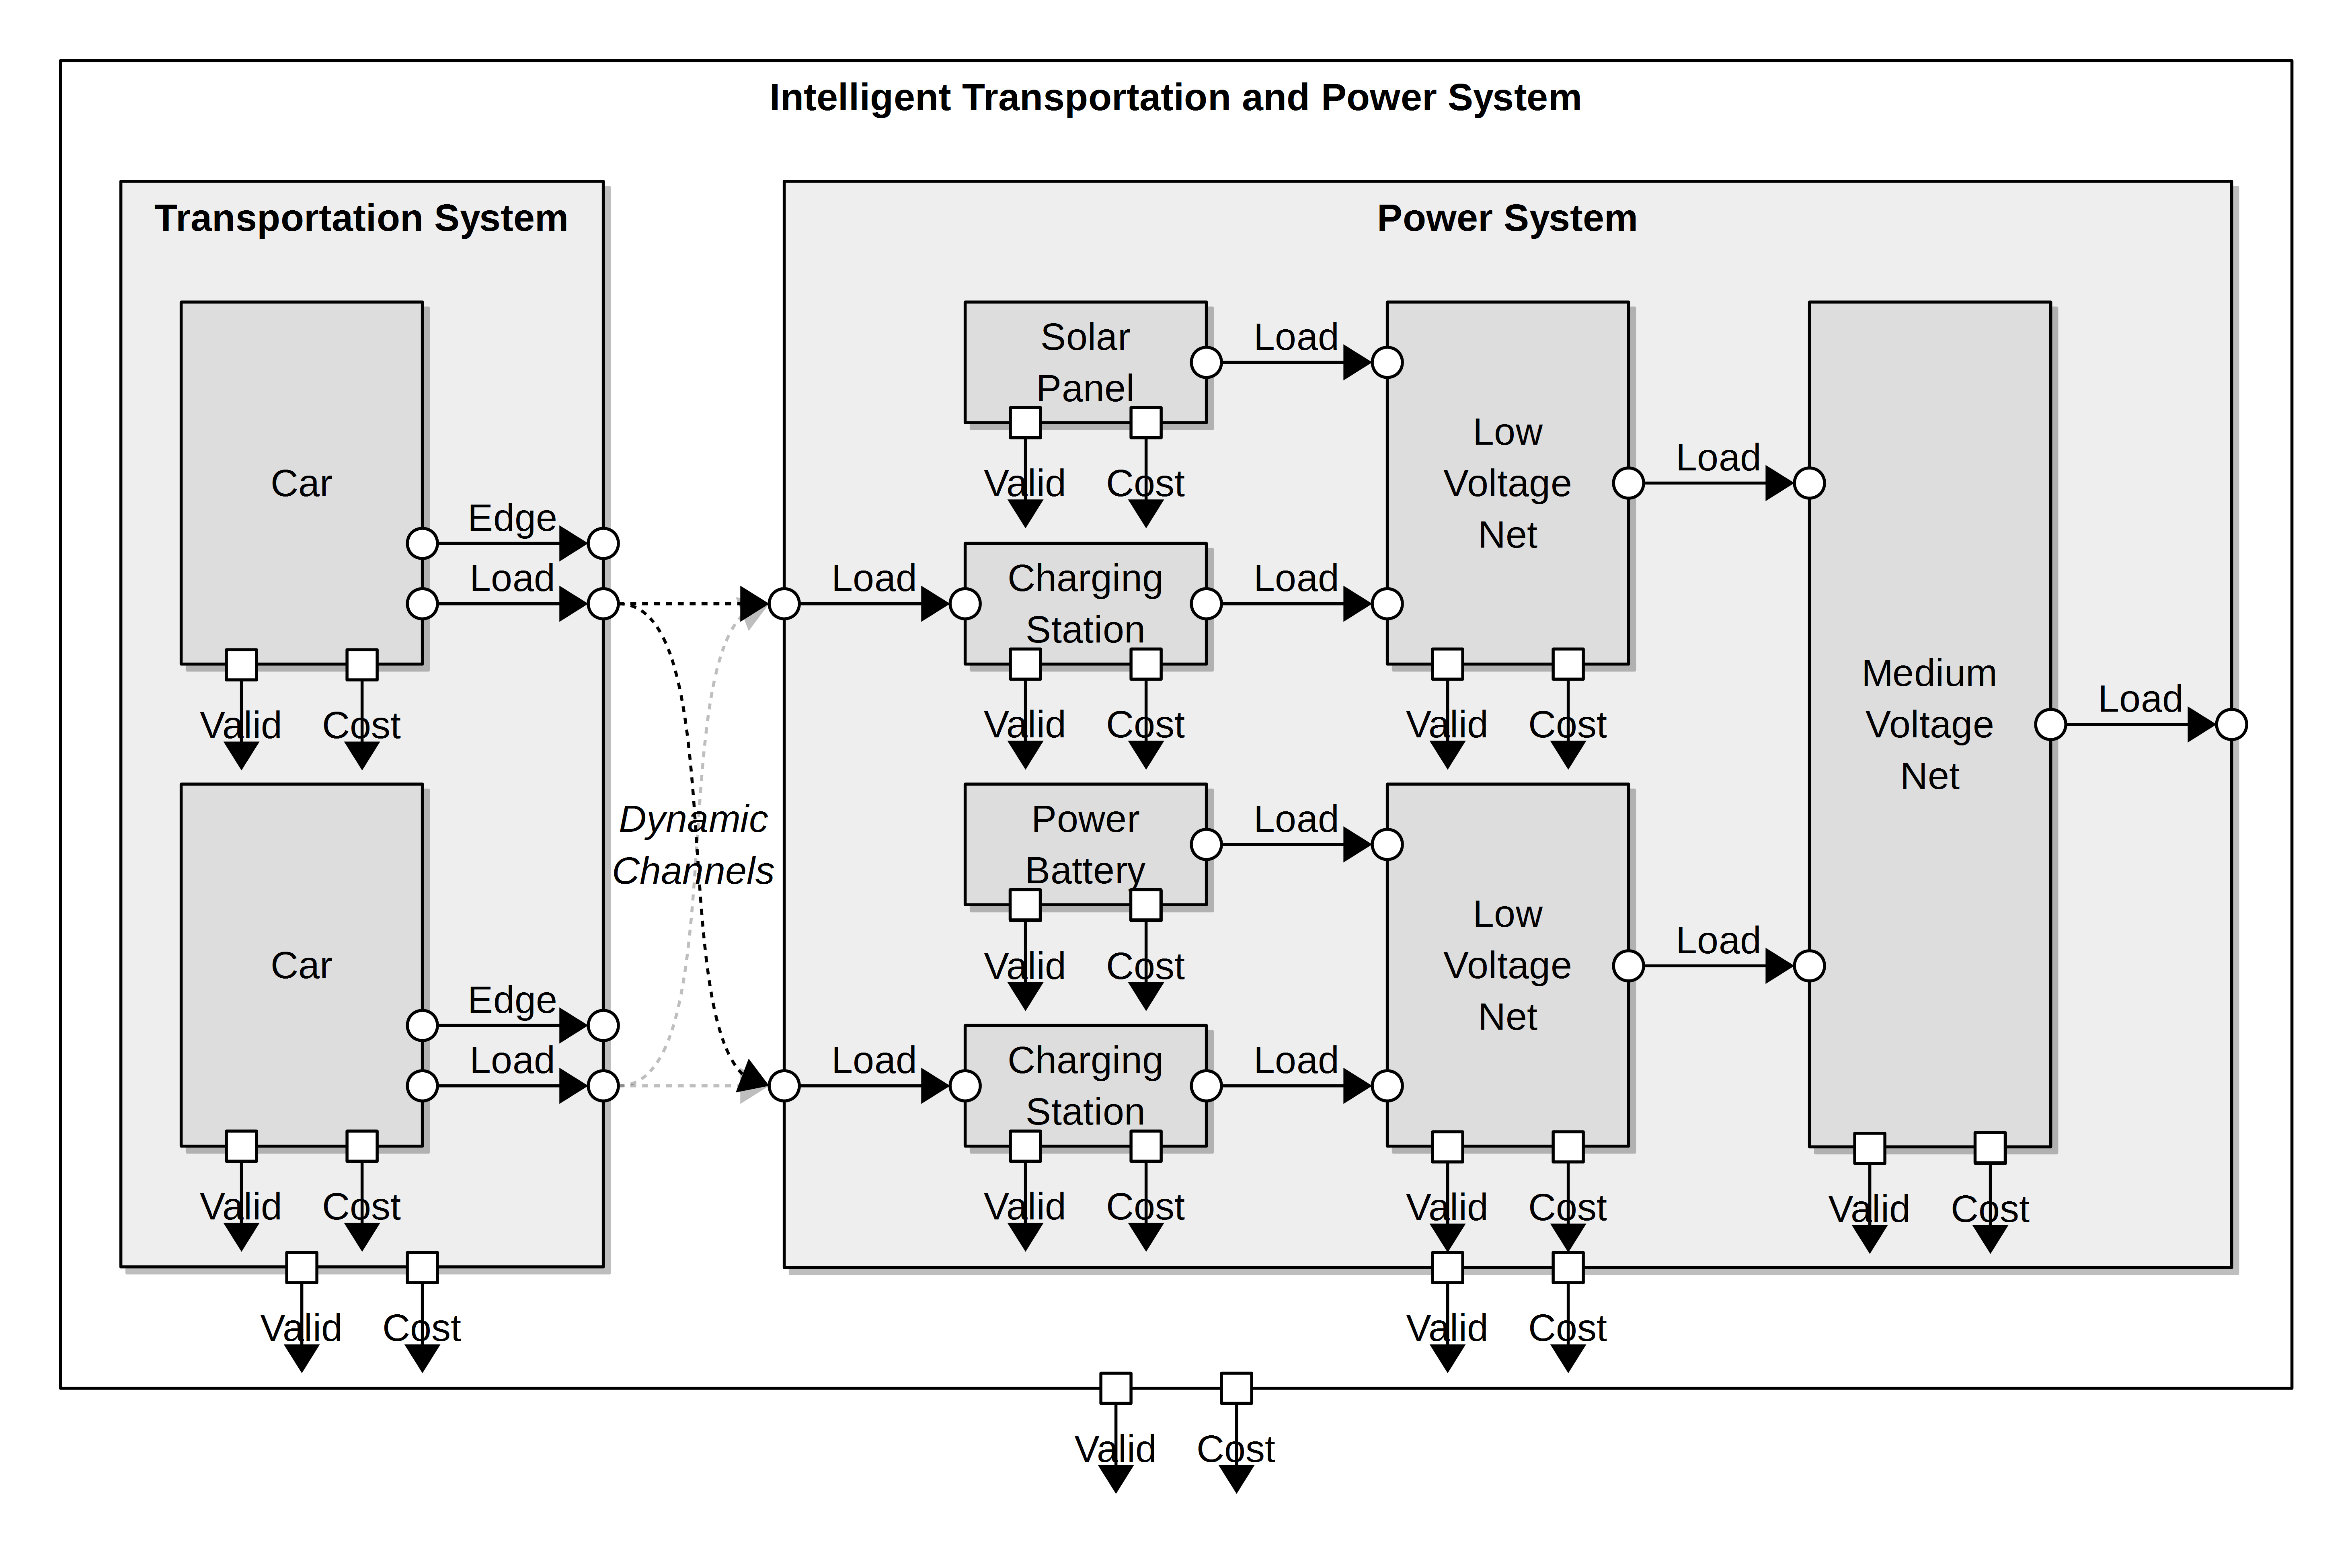
\includegraphics[width=\columnwidth]{../gfx/example.png}
		\caption{Example 1}
		\label{figure:examples_1}
	\end{subfigure}
	\hfill
	\begin{subfigure}{\columnwidth}
		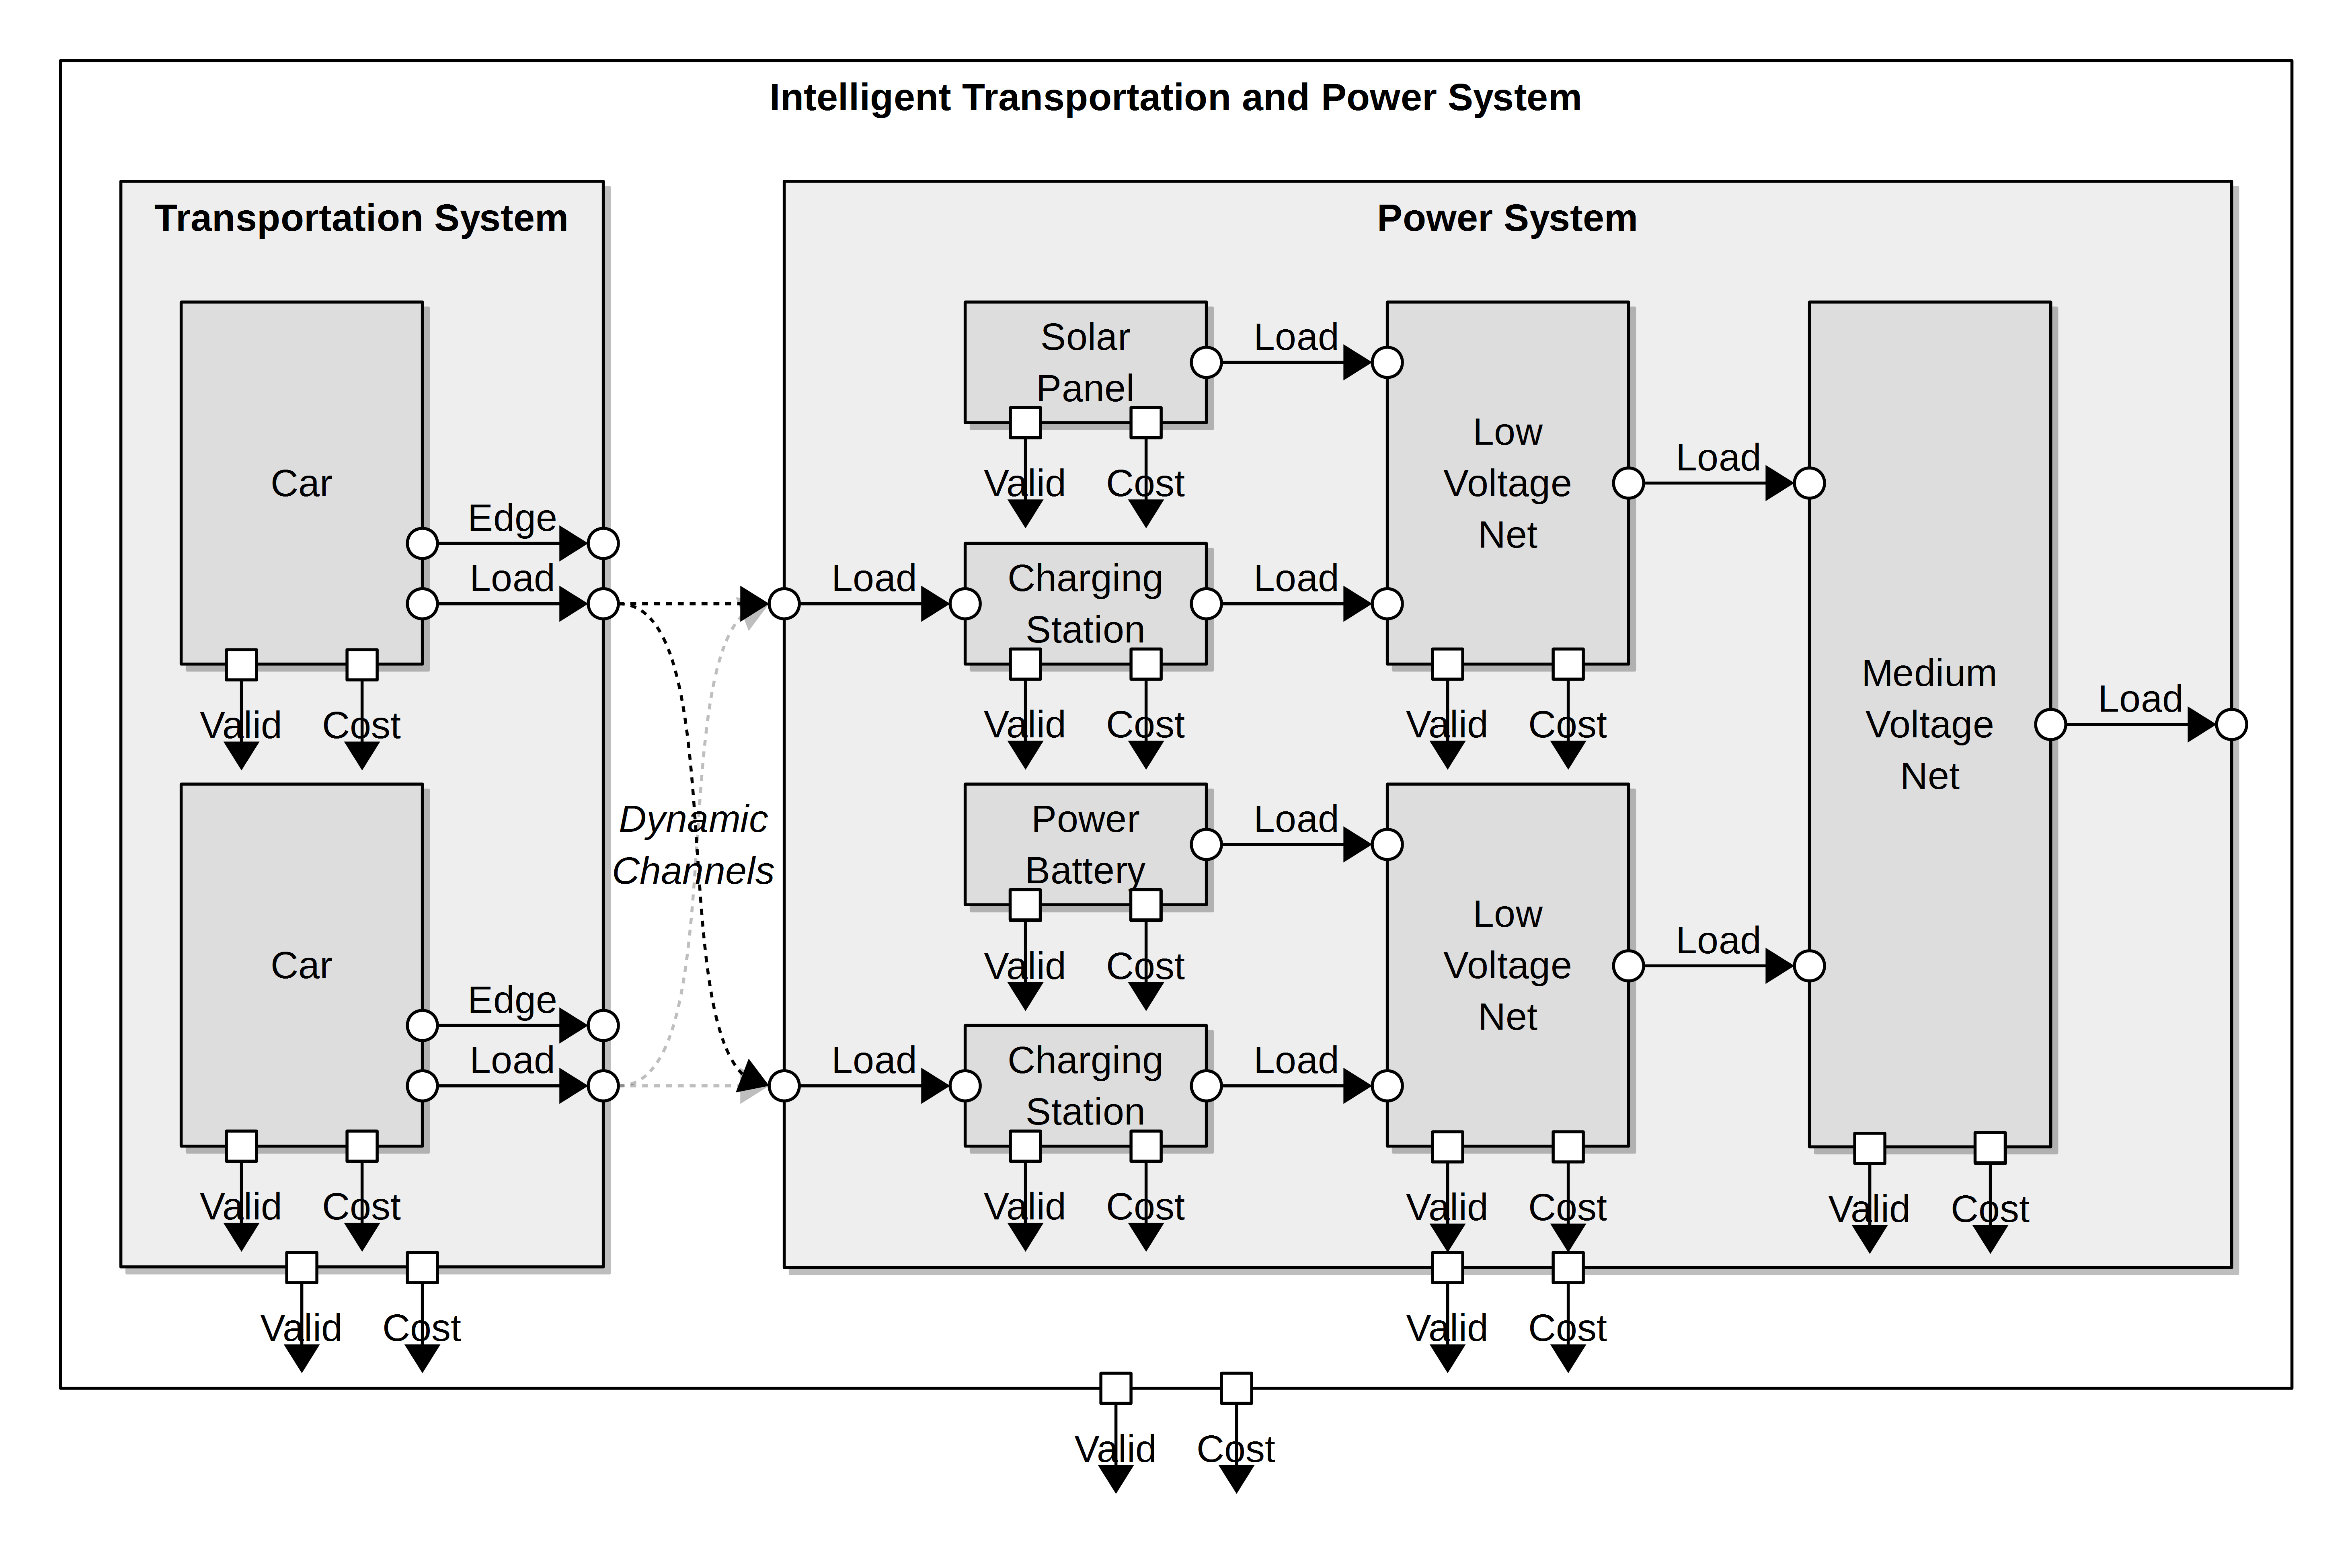
\includegraphics[width=\columnwidth]{../gfx/example.png}
		\caption{Example 2}
		\label{figure:examples_2}
	\end{subfigure}
	
	\begin{subfigure}{\columnwidth}
		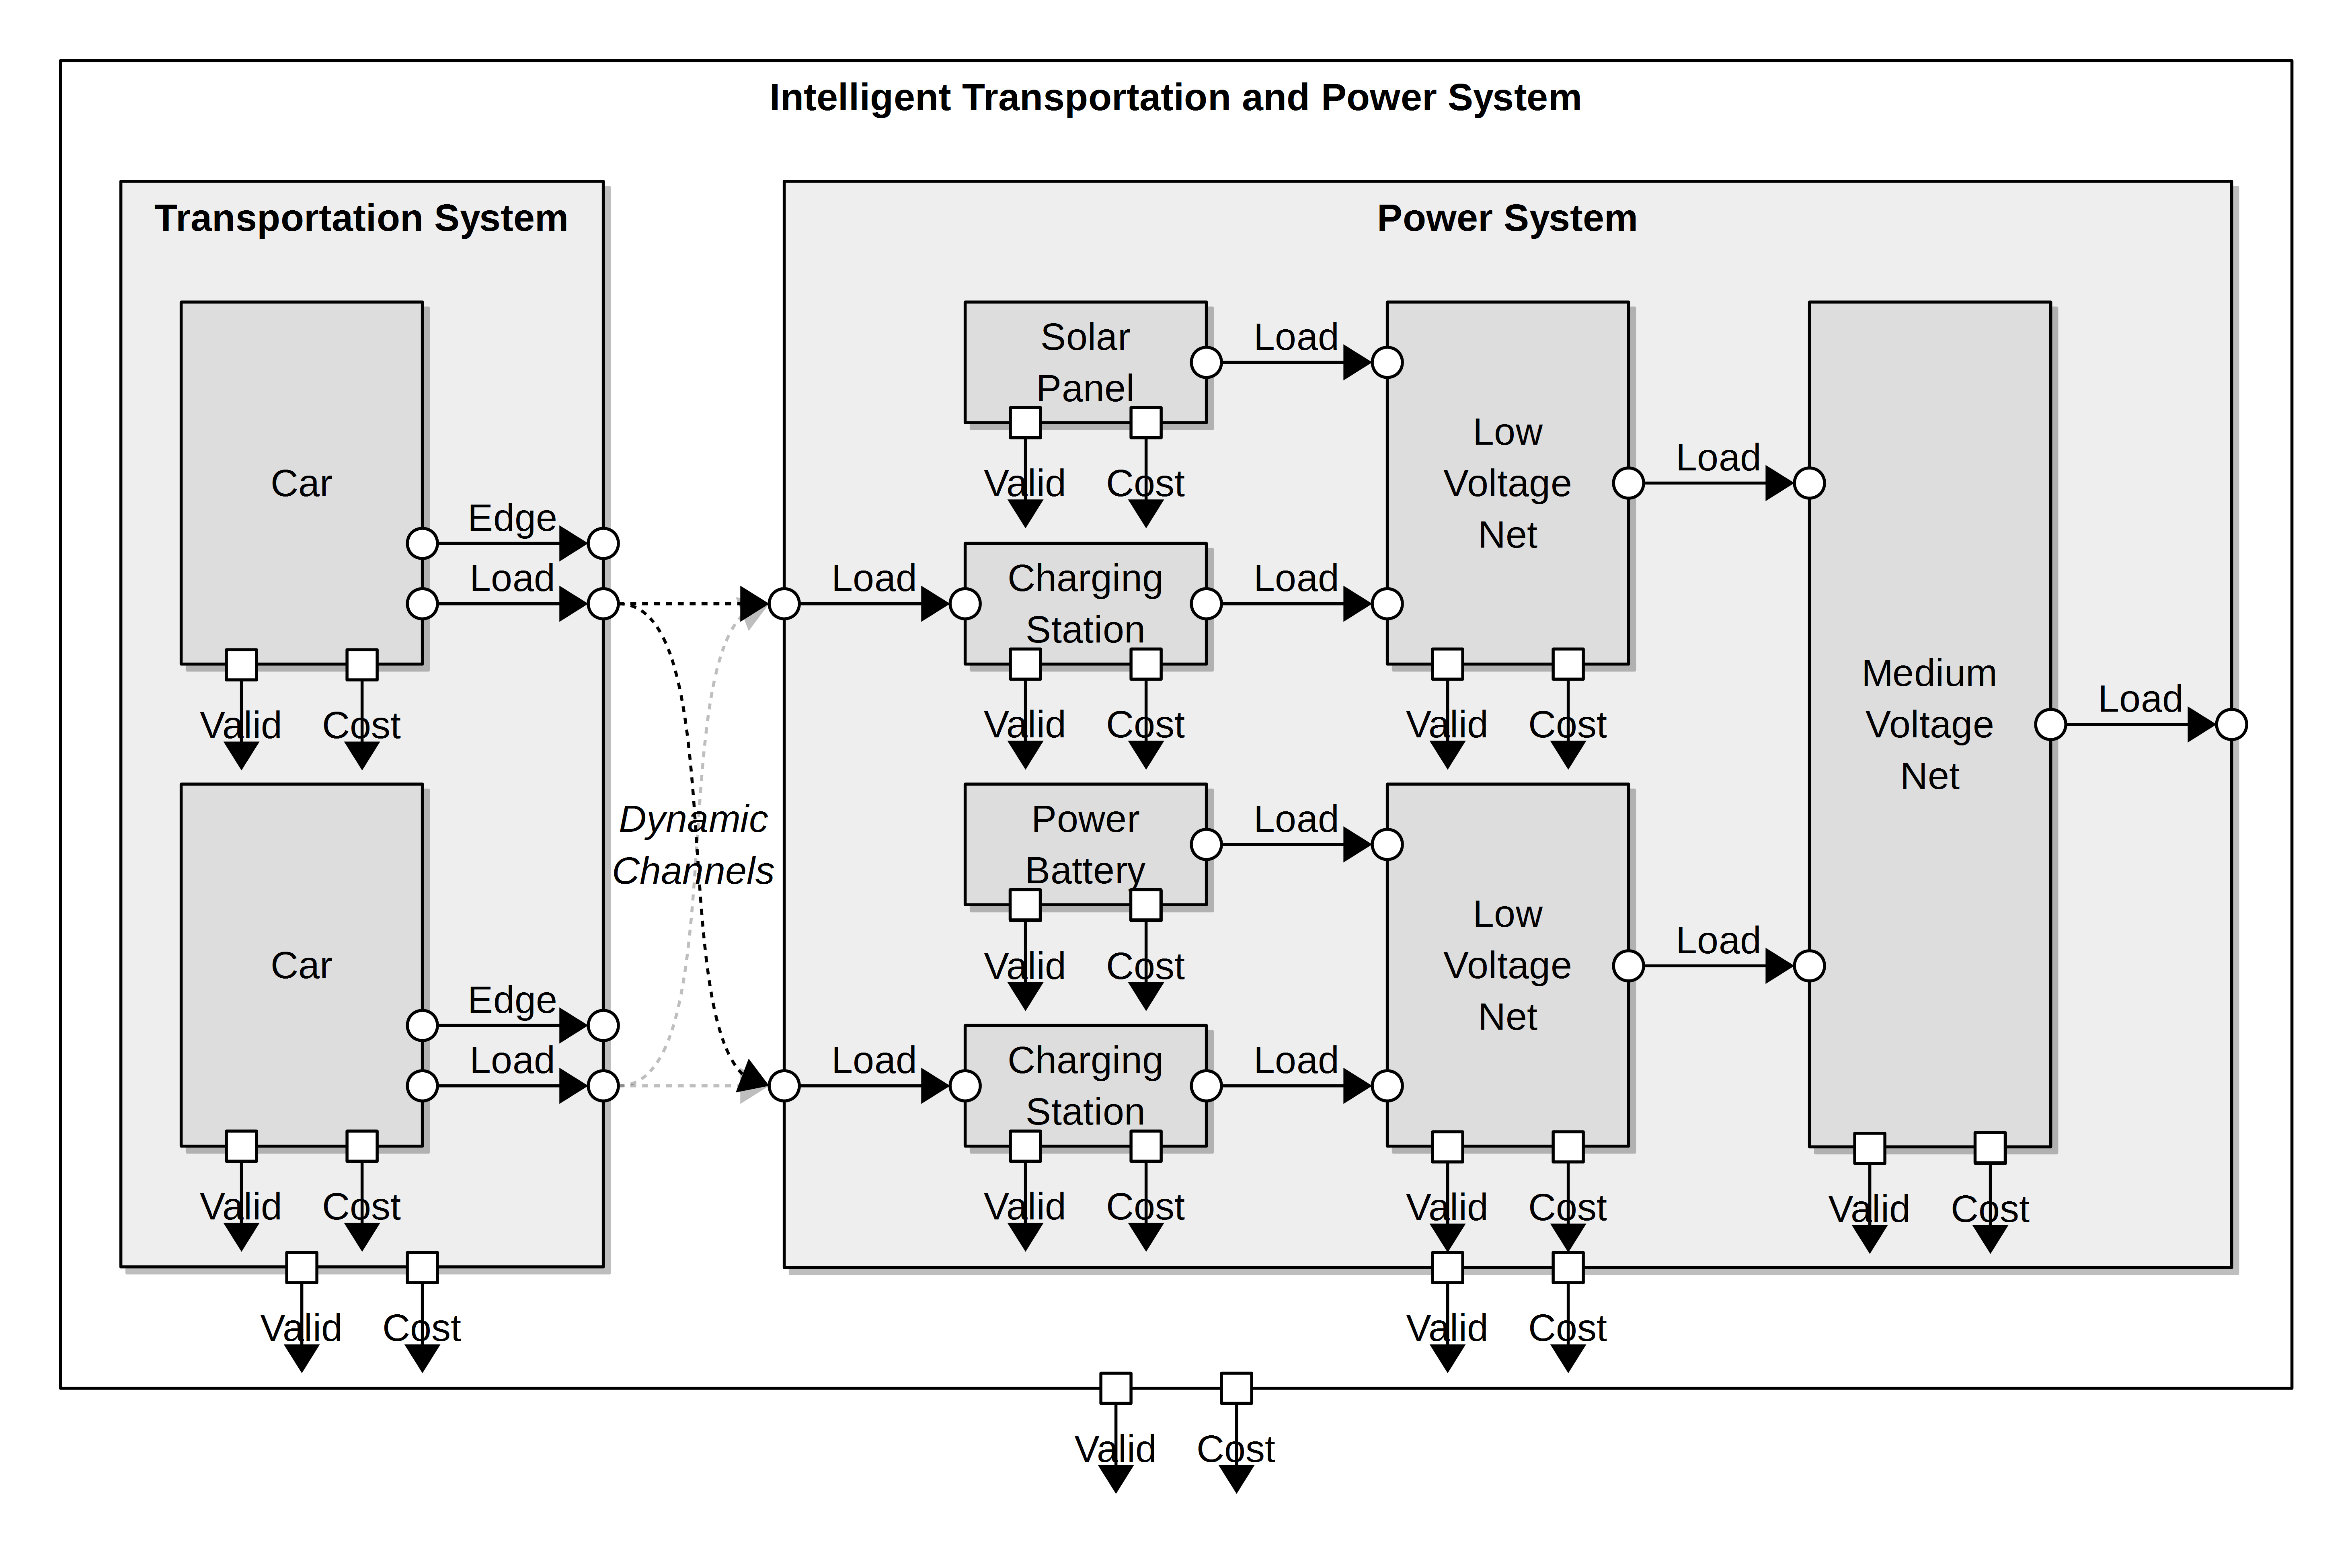
\includegraphics[width=\columnwidth]{../gfx/example.png}
		\caption{Example 3}
		\label{figure:examples_3}
	\end{subfigure}
	\hfill
	\begin{subfigure}{\columnwidth}
		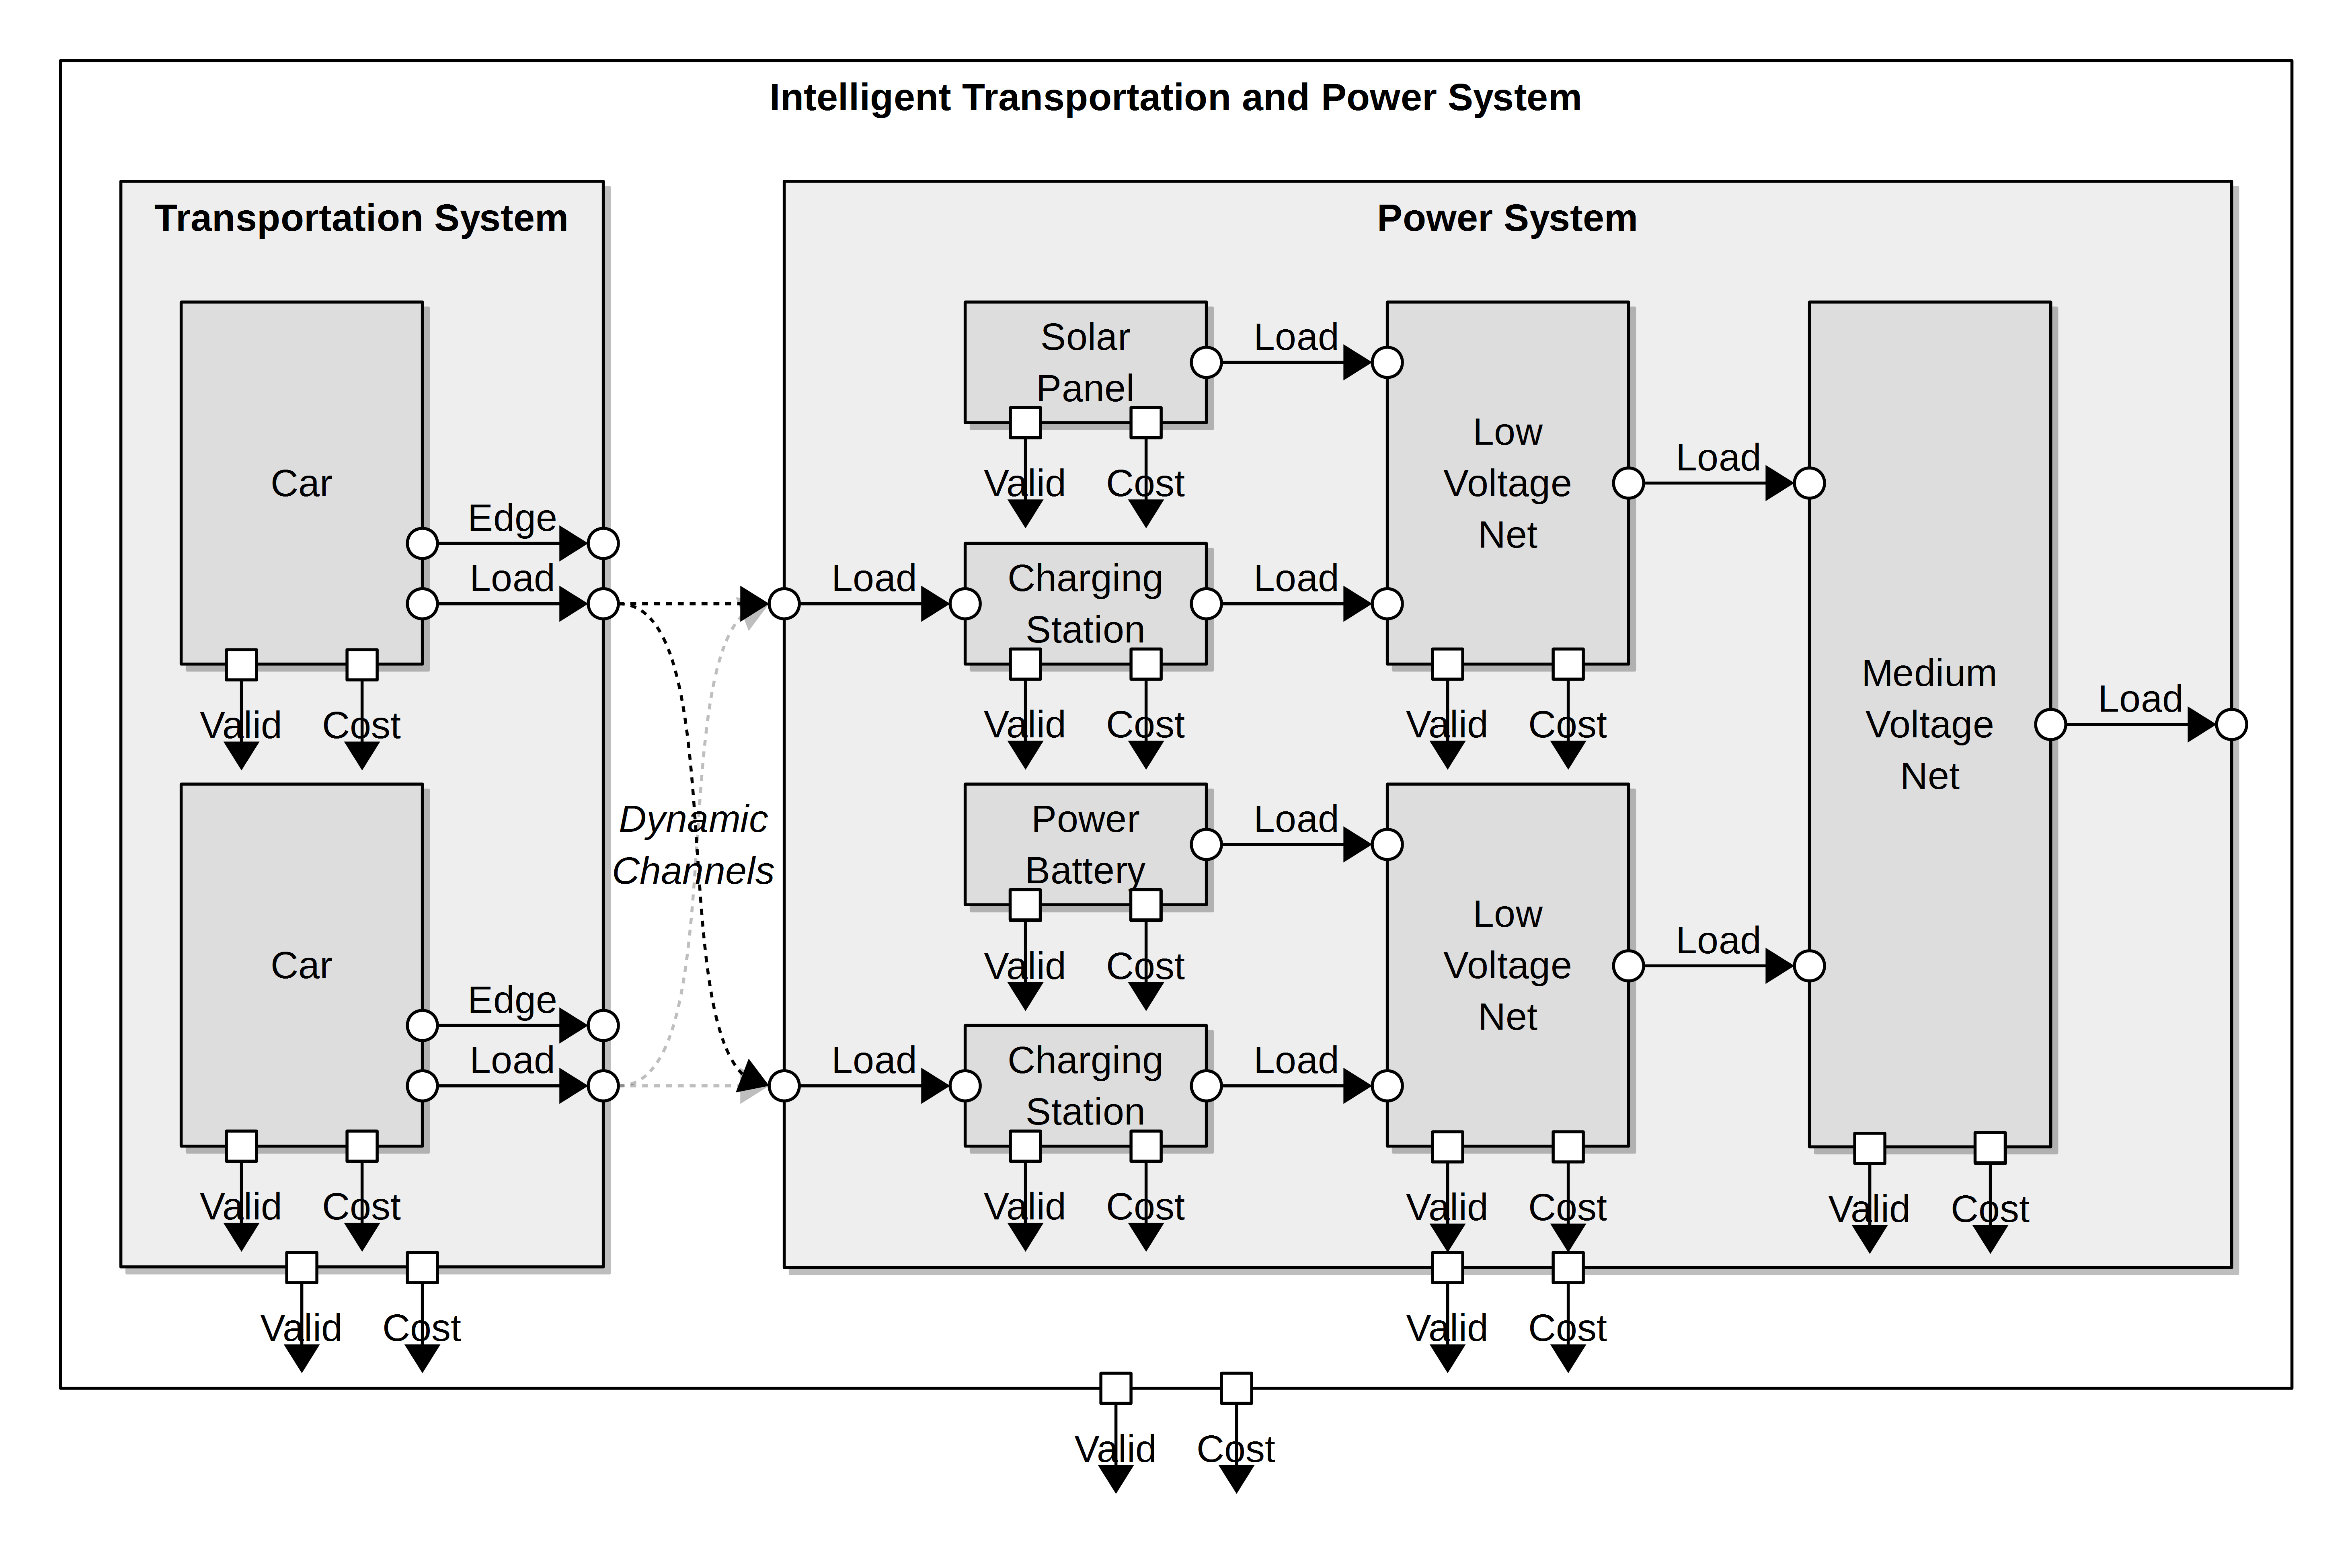
\includegraphics[width=\columnwidth]{../gfx/example.png}
		\caption{Example 4}
		\label{figure:examples_4}
	\end{subfigure}
	
	\caption{Examples.}
	\label{figure:examples}
\end{figure*}

TBD

\subsection{Discussion}
\label{section:discussion}

TBD